\documentclass[11pt,a4paper]{article}
\usepackage[margin=1.9cm, top=2.1cm, bottom=2.0cm]{geometry}
\usepackage[T1]{fontenc}
\usepackage{lmodern}
\usepackage{amsmath,amssymb}
\usepackage{enumitem,booktabs,array,tabularx,multirow}
\usepackage[normalem]{ulem}
\usepackage{adjustbox}
\usepackage{xcolor}
\usepackage{fancyhdr,lastpage}
\usepackage[most]{tcolorbox}
\usepackage{tikz}
\usetikzlibrary{shapes.geometric,arrows.meta,positioning,calc}
\usepackage[hidelinks]{hyperref}
\setlength{\parindent}{0pt}
\setlength{\parskip}{4pt}
\renewcommand{\arraystretch}{1.25}
\emergencystretch=2em
\pagestyle{fancy}\fancyhf{}
\lhead{\small\textit{Course: CS420 -- Artificial Intelligence}}
\rhead{\small Practice Test 2}
\cfoot{\small Page \thepage\ of \pageref{LastPage}}
\renewcommand{\headrulewidth}{0.4pt}
% empty answer box (exam) / filled box (solution)
\newtcolorbox{ansbox}[1][]{enhanced, breakable, colback=white, colframe=black!55, boxrule=0.5pt, arc=0pt,
  left=5pt, right=5pt, top=3pt, bottom=3pt, before skip=3pt, after skip=6pt, #1}
\newtcolorbox{solbox}{enhanced, breakable, colback=blue!2!white, colframe=blue!50!black, boxrule=0.6pt, arc=0pt,
  left=6pt, right=6pt, top=4pt, bottom=4pt, before skip=3pt, after skip=8pt,
  fontupper=\color{black}}
\newcommand{\question}[1]{\par\medskip\noindent\textbf{Question #1.}\ }
\newcommand{\subq}[1]{\par\smallskip\noindent\textbf{#1}\ }
\newcommand{\T}{\textbf{\textcolor{green!45!black}{TRUE}}}
\newcommand{\F}{\textbf{\textcolor{red!70!black}{FALSE}}}

\tikzset{
  maxn/.style={draw, thick, regular polygon, regular polygon sides=3, minimum size=10.5mm, inner sep=0pt, font=\small},
  minn/.style={maxn, shape border rotate=180},
  chn/.style={draw, thick, circle, minimum size=9.5mm, inner sep=0pt, font=\small},
  leafn/.style={draw, rectangle, minimum width=5.5mm, minimum height=5.5mm, inner sep=1pt, font=\small},
  gone/.style={draw=black!25, text=black!35},
  cut/.style={red!80!black, very thick, dashed},
  sol/.style={text=blue!70!black, font=\small\bfseries},
}

\begin{document}


{\large\textbf{\textit{Course: CS420 -- Artificial Intelligence}}}\par
{\textbf{\textit{Midterm examination review -- Lectures 0 to 3}}}\par
\begin{center}{\Large\bfseries PRACTICE MIDTERM EXAMINATION -- TEST 2}\\[3pt]
{\small Duration: 120 minutes \quad$\cdot$\quad Closed book \quad$\cdot$\quad Calculator allowed}\end{center}
\noindent\rule{\linewidth}{0.6pt}

\noindent Full name: \rule{6.5cm}{0.3pt}\hfill Student ID: \rule{4cm}{0.3pt}\par\smallskip
{\small\textit{Unless a question says otherwise, ties are broken in alphabetical order (left-to-right in trees), and successors are generated in alphabetical order.}}\par
\question{1}\textit{Farmer, wolf, goat and cabbage.} A farmer must take a wolf, a goat and a cabbage across a river. The boat holds the farmer and at most one of the three items, and only the farmer can row. Left unattended (without the farmer), the wolf eats the goat and the goat eats the cabbage.
\subq{(a)}Consider a state as a tuple of values. Which values should be included in the tuple?
\begin{ansbox}[height=1.0cm]\end{ansbox}
\subq{(b)}Define the initial state and the goal state.
\begin{ansbox}[height=0.8cm]\end{ansbox}
\subq{(c)}Define the action function.
\begin{ansbox}[height=1.8cm]\end{ansbox}
\subq{(d)}What is the action cost?
\begin{ansbox}[height=0.6cm]\end{ansbox}
\subq{(e)}What is the maximum number of states (including illegal ones)? How many states are legal, and how many are reachable? Give a shortest solution.
\begin{ansbox}[height=2.0cm]\end{ansbox}
\question{2}Consider the \emph{directed} graph below; $S$ is the initial state and $G$ the goal state. \begin{center}
\begin{adjustbox}{max width=\linewidth}
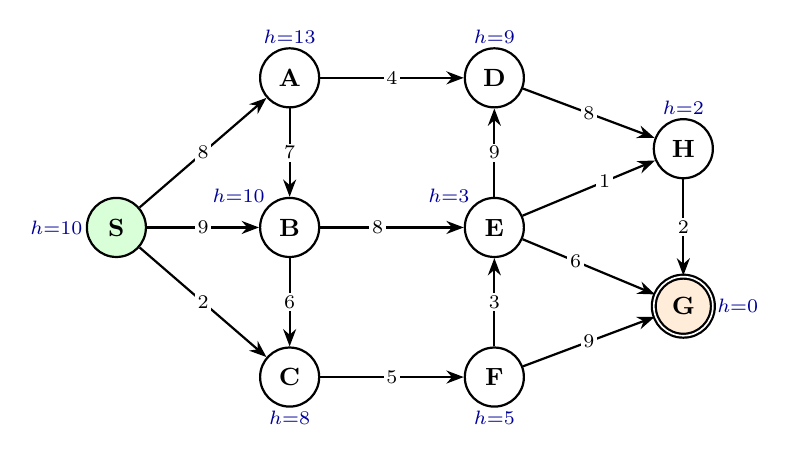
\begin{tikzpicture}[scale=1.0, every node/.style={transform shape}, gn/.style={draw, thick, circle, minimum size=7.5mm, inner sep=0pt, font=\small\bfseries}, ec/.style={font=\scriptsize, fill=white, inner sep=1pt}]
\node[gn, fill=green!15, label={[font=\scriptsize, text=blue!60!black, inner sep=1pt]left:$h{=}10$}] (S) at (0.00,0.00) {S};
\node[gn, label={[font=\scriptsize, text=blue!60!black, inner sep=1pt]above:$h{=}13$}] (A) at (2.20,1.90) {A};
\node[gn, label={[font=\scriptsize, text=blue!60!black, inner sep=1pt]above left:$h{=}10$}] (B) at (2.20,0.00) {B};
\node[gn, label={[font=\scriptsize, text=blue!60!black, inner sep=1pt]below:$h{=}8$}] (C) at (2.20,-1.90) {C};
\node[gn, label={[font=\scriptsize, text=blue!60!black, inner sep=1pt]above:$h{=}9$}] (D) at (4.80,1.90) {D};
\node[gn, label={[font=\scriptsize, text=blue!60!black, inner sep=1pt]above left:$h{=}3$}] (E) at (4.80,0.00) {E};
\node[gn, label={[font=\scriptsize, text=blue!60!black, inner sep=1pt]below:$h{=}5$}] (F) at (4.80,-1.90) {F};
\node[gn, label={[font=\scriptsize, text=blue!60!black, inner sep=1pt]above:$h{=}2$}] (H) at (7.20,1.00) {H};
\node[gn, double, fill=orange!15, label={[font=\scriptsize, text=blue!60!black, inner sep=1pt]right:$h{=}0$}] (G) at (7.20,-1.00) {G};
\draw[thick,-{Stealth[length=2.2mm]}] (S) to[] node[ec, midway]{8} (A);
\draw[thick,-{Stealth[length=2.2mm]}] (S) to[] node[ec, midway]{9} (B);
\draw[thick,-{Stealth[length=2.2mm]}] (S) to[] node[ec, midway]{2} (C);
\draw[thick,-{Stealth[length=2.2mm]}] (A) to[] node[ec, midway]{4} (D);
\draw[thick,-{Stealth[length=2.2mm]}] (A) to[] node[ec, midway]{7} (B);
\draw[thick,-{Stealth[length=2.2mm]}] (B) to[] node[ec, pos=0.4]{8} (E);
\draw[thick,-{Stealth[length=2.2mm]}] (C) to[] node[ec, midway]{5} (F);
\draw[thick,-{Stealth[length=2.2mm]}] (B) to[] node[ec, midway]{6} (C);
\draw[thick,-{Stealth[length=2.2mm]}] (D) to[] node[ec, midway]{8} (H);
\draw[thick,-{Stealth[length=2.2mm]}] (E) to[] node[ec, midway]{9} (D);
\draw[thick,-{Stealth[length=2.2mm]}] (E) to[] node[ec, pos=0.4]{6} (G);
\draw[thick,-{Stealth[length=2.2mm]}] (F) to[] node[ec, midway]{3} (E);
\draw[thick,-{Stealth[length=2.2mm]}] (F) to[] node[ec, midway]{9} (G);
\draw[thick,-{Stealth[length=2.2mm]}] (H) to[] node[ec, midway]{2} (G);
\draw[thick,-{Stealth[length=2.2mm]}] (E) to[] node[ec, pos=0.62]{1} (H);
\end{tikzpicture}
\end{adjustbox}
\end{center}For each search strategy, (a) list, in order, the states \textbf{expanded}, (b) give the path found and (c) give the final content of the frontier (a state is expanded when it is removed from the frontier). Conventions: BFS, DFS and greedy best-first search test a state for the goal when it is \emph{generated} (so the goal is not expanded); UCS and A* test it when it is \emph{removed} from the frontier (graph search; a cheaper path to a frontier state replaces its entry). DFS avoids loops by remembering the states on the current path only. The path returned will not be accepted if the list of expanded states is wrong.

\begin{center}\small\begin{tabularx}{\linewidth}{|>{\raggedright}p{2.6cm}|>{\raggedright}X|>{\raggedright}p{3.6cm}|>{\raggedright\arraybackslash}p{2.6cm}|}\hline
\textbf{Algorithm} & \textbf{List of expanded states} & \textbf{Path returned} & \textbf{Final frontier}\\ \hline
Breadth-first search & & & \\[8mm] \hline
Uniform-cost search & & & \\[8mm] \hline
Depth-first search & & & \textit{(not asked)}\\[8mm] \hline
Greedy best-first search & & & \\[8mm] \hline
Graph-search A* & & & \\[8mm] \hline
\end{tabularx}\end{center}
\subq{(d)}Is $h$ admissible? Is it consistent? Justify (only the direction of each edge matters).
\begin{ansbox}[height=1.8cm]\end{ansbox}
\subq{(e)}UCS and A* return the same path. Why does A* expand fewer states?
\begin{ansbox}[height=1.5cm]\end{ansbox}
\clearpage
\question{3}\textit{4-bishops.} Consider the 4-bishops problem: every state has 4 bishops on a $4\times4$ board, one in each column. A bishop attacks along the diagonals (count attacking pairs regardless of pieces in between).\begin{center}
\begin{adjustbox}{max width=\linewidth}
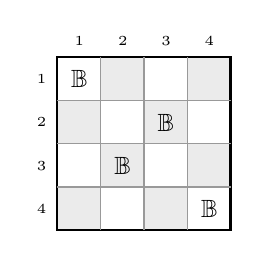
\begin{tikzpicture}
\fill[white] (0.00,0.00) rectangle +(0.55,-0.55);
\fill[black!8] (0.00,-0.55) rectangle +(0.55,-0.55);
\fill[white] (0.00,-1.10) rectangle +(0.55,-0.55);
\fill[black!8] (0.00,-1.65) rectangle +(0.55,-0.55);
\fill[black!8] (0.55,0.00) rectangle +(0.55,-0.55);
\fill[white] (0.55,-0.55) rectangle +(0.55,-0.55);
\fill[black!8] (0.55,-1.10) rectangle +(0.55,-0.55);
\fill[white] (0.55,-1.65) rectangle +(0.55,-0.55);
\fill[white] (1.10,0.00) rectangle +(0.55,-0.55);
\fill[black!8] (1.10,-0.55) rectangle +(0.55,-0.55);
\fill[white] (1.10,-1.10) rectangle +(0.55,-0.55);
\fill[black!8] (1.10,-1.65) rectangle +(0.55,-0.55);
\fill[black!8] (1.65,0.00) rectangle +(0.55,-0.55);
\fill[white] (1.65,-0.55) rectangle +(0.55,-0.55);
\fill[black!8] (1.65,-1.10) rectangle +(0.55,-0.55);
\fill[white] (1.65,-1.65) rectangle +(0.55,-0.55);
\draw[thick] (0,0) rectangle (2.20,-2.20);
\draw[black!40] (0.55,0) -- (0.55,-2.20);
\draw[black!40] (0,-0.55) -- (2.20,-0.55);
\draw[black!40] (1.10,0) -- (1.10,-2.20);
\draw[black!40] (0,-1.10) -- (2.20,-1.10);
\draw[black!40] (1.65,0) -- (1.65,-2.20);
\draw[black!40] (0,-1.65) -- (2.20,-1.65);
\node[font=\small\bfseries] at (0.28,-0.28) {$\mathbb{B}$};
\node[font=\small\bfseries] at (0.83,-1.38) {$\mathbb{B}$};
\node[font=\small\bfseries] at (1.38,-0.83) {$\mathbb{B}$};
\node[font=\small\bfseries] at (1.93,-1.93) {$\mathbb{B}$};
\node[font=\tiny] at (0.28,0.20) {1};
\node[font=\tiny] at (0.83,0.20) {2};
\node[font=\tiny] at (1.38,0.20) {3};
\node[font=\tiny] at (1.93,0.20) {4};
\node[font=\tiny] at (-0.20,-0.28) {1};
\node[font=\tiny] at (-0.20,-0.83) {2};
\node[font=\tiny] at (-0.20,-1.38) {3};
\node[font=\tiny] at (-0.20,-1.93) {4};
\end{tikzpicture}
\end{adjustbox}
\end{center}
\subq{(a)}What is the total number of states in the state space? Explain.
\begin{ansbox}[height=0.9cm]\end{ansbox}
\subq{(b)}Each step moves one bishop within its own column. How many successors does a state have? Explain.
\begin{ansbox}[height=0.9cm]\end{ansbox}
\subq{(c)}A state is written as 4 digits giving the row of the bishop in columns 1--4 (the board above is 1324). Let $n_b$ be the number of attacking pairs of bishops of state $n$. Define a fitness function Fit$(n)$ to be maximised by the genetic algorithm.
\begin{ansbox}[height=0.9cm]\end{ansbox}
\subq{(d)}The current generation is $S_1=1324$, $S_2=2143$, $S_3=3412$, $S_4=4132$. Compute Fit$(n)$ and the probability that each state is chosen in the roulette-wheel selection step. Then cross $S_1$ with $S_4$ after the 2nd digit and give the two children with their fitness.
\begin{center}\begin{tabular}{|l|c|c|c|c|}\hline State $n$ & $S_1=1324$ & $S_2=2143$ & $S_3=3412$ & $S_4=4132$\\\hline Fit$(n)$ & & & & \\[2mm]\hline Prob$(n)$ & & & & \\[2mm]\hline\end{tabular}\end{center}\begin{ansbox}[height=1.2cm]\end{ansbox}
\clearpage
\question{4}Consider the following game tree. The root is a MAX node; children are visited left to right.\begin{center}
\begin{adjustbox}{max width=\linewidth}
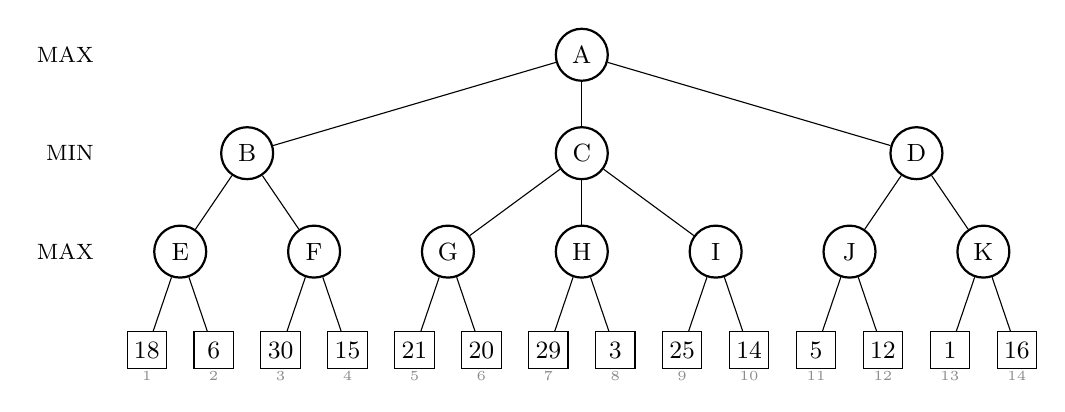
\begin{tikzpicture}[scale=1.0, every node/.style={transform shape}, gc/.style={draw, thick, circle, minimum size=6.6mm, inner sep=0pt, font=\small}, gl/.style={draw, rectangle, minimum width=5mm, minimum height=4.6mm, inner sep=1pt, font=\small}, gx/.style={draw=black!25, text=black!35}, val/.style={font=\footnotesize\bfseries, text=red!80!black, inner sep=1pt}]
\node[font=\footnotesize, anchor=east] at (-0.55,0.00) {MAX};
\node[font=\footnotesize, anchor=east] at (-0.55,-1.25) {MIN};
\node[font=\footnotesize, anchor=east] at (-0.55,-2.50) {MAX};
\node[gc] (n24) at (5.525,0.000) {A};
\node[gc] (n6) at (1.275,-1.250) {B};
\node[gc] (n2) at (0.425,-2.500) {E};
\node[gl, label={[font=\tiny, text=black!45, inner sep=1pt]below:1}] (n0) at (0.000,-3.750) {18};
\node[gl, label={[font=\tiny, text=black!45, inner sep=1pt]below:2}] (n1) at (0.850,-3.750) {6};
\node[gc] (n5) at (2.125,-2.500) {F};
\node[gl, label={[font=\tiny, text=black!45, inner sep=1pt]below:3}] (n3) at (1.700,-3.750) {30};
\node[gl, label={[font=\tiny, text=black!45, inner sep=1pt]below:4}] (n4) at (2.550,-3.750) {15};
\node[gc] (n16) at (5.525,-1.250) {C};
\node[gc] (n9) at (3.825,-2.500) {G};
\node[gl, label={[font=\tiny, text=black!45, inner sep=1pt]below:5}] (n7) at (3.400,-3.750) {21};
\node[gl, label={[font=\tiny, text=black!45, inner sep=1pt]below:6}] (n8) at (4.250,-3.750) {20};
\node[gc] (n12) at (5.525,-2.500) {H};
\node[gl, label={[font=\tiny, text=black!45, inner sep=1pt]below:7}] (n10) at (5.100,-3.750) {29};
\node[gl, label={[font=\tiny, text=black!45, inner sep=1pt]below:8}] (n11) at (5.950,-3.750) {3};
\node[gc] (n15) at (7.225,-2.500) {I};
\node[gl, label={[font=\tiny, text=black!45, inner sep=1pt]below:9}] (n13) at (6.800,-3.750) {25};
\node[gl, label={[font=\tiny, text=black!45, inner sep=1pt]below:10}] (n14) at (7.650,-3.750) {14};
\node[gc] (n23) at (9.775,-1.250) {D};
\node[gc] (n19) at (8.925,-2.500) {J};
\node[gl, label={[font=\tiny, text=black!45, inner sep=1pt]below:11}] (n17) at (8.500,-3.750) {5};
\node[gl, label={[font=\tiny, text=black!45, inner sep=1pt]below:12}] (n18) at (9.350,-3.750) {12};
\node[gc] (n22) at (10.625,-2.500) {K};
\node[gl, label={[font=\tiny, text=black!45, inner sep=1pt]below:13}] (n20) at (10.200,-3.750) {1};
\node[gl, label={[font=\tiny, text=black!45, inner sep=1pt]below:14}] (n21) at (11.050,-3.750) {16};
\draw (n24) -- (n6);
\draw (n24) -- (n16);
\draw (n24) -- (n23);
\draw (n6) -- (n2);
\draw (n6) -- (n5);
\draw (n2) -- (n0);
\draw (n2) -- (n1);
\draw (n5) -- (n3);
\draw (n5) -- (n4);
\draw (n16) -- (n9);
\draw (n16) -- (n12);
\draw (n16) -- (n15);
\draw (n9) -- (n7);
\draw (n9) -- (n8);
\draw (n12) -- (n10);
\draw (n12) -- (n11);
\draw (n15) -- (n13);
\draw (n15) -- (n14);
\draw (n23) -- (n19);
\draw (n23) -- (n22);
\draw (n19) -- (n17);
\draw (n19) -- (n18);
\draw (n22) -- (n20);
\draw (n22) -- (n21);
\end{tikzpicture}
\end{adjustbox}
\end{center}
\subq{(a)}Compute the final backed-up value of every node using the minimax algorithm (no alpha-beta pruning at this step). Which move should MAX make at the root?
\begin{center}\small \begin{tabular}{|l|c|c|c|c|c|c|c|c|c|c|c|}\hline
\textbf{Node} & \textbf{A} & \textbf{B} & \textbf{C} & \textbf{D} & \textbf{E} & \textbf{F} & \textbf{G} & \textbf{H} & \textbf{I} & \textbf{J} & \textbf{K}\\ \hline
Minimax & \phantom{00} & \phantom{00} & \phantom{00} & \phantom{00} & \phantom{00} & \phantom{00} & \phantom{00} & \phantom{00} & \phantom{00} & \phantom{00} & \phantom{00}\\[1.5mm] \hline
\end{tabular}\end{center}\begin{ansbox}[height=0.8cm]\end{ansbox}
\subq{(b)}Run alpha-beta pruning (children visited left to right). Give the value computed at every node (mark \textbf{X} if the node is never visited), cross out the pruned branches on the tree and briefly explain each case.
\begin{center}\small \begin{tabular}{|l|c|c|c|c|c|c|c|c|c|c|c|}\hline
\textbf{Node} & \textbf{A} & \textbf{B} & \textbf{C} & \textbf{D} & \textbf{E} & \textbf{F} & \textbf{G} & \textbf{H} & \textbf{I} & \textbf{J} & \textbf{K}\\ \hline
$\alpha$-$\beta$ & \phantom{00} & \phantom{00} & \phantom{00} & \phantom{00} & \phantom{00} & \phantom{00} & \phantom{00} & \phantom{00} & \phantom{00} & \phantom{00} & \phantom{00}\\[1.5mm] \hline
\end{tabular}\end{center}\begin{ansbox}[height=4.0cm]\end{ansbox}
\subq{(c)}Using the minimax values from (a), and without performing any alpha-beta calculation, rotate the children of each node at every level so that alpha-beta prunes as much as possible. Draw the new tree (keep the node letters).
\begin{ansbox}[height=5.5cm]\end{ansbox}
\clearpage
\question{5}Consider the game tree below, in which \textbf{MIN moves first} (the root is a MIN node).\begin{center}
\begin{adjustbox}{max width=\linewidth}
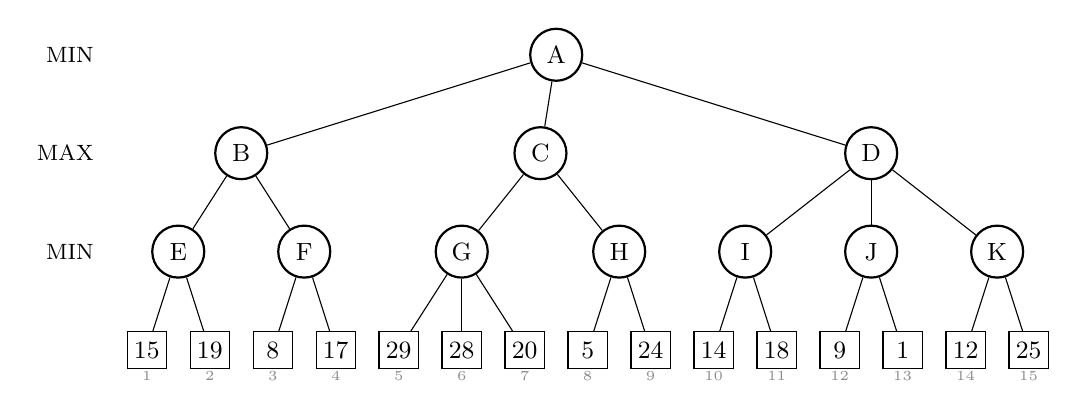
\begin{tikzpicture}[scale=1.0, every node/.style={transform shape}, gc/.style={draw, thick, circle, minimum size=6.6mm, inner sep=0pt, font=\small}, gl/.style={draw, rectangle, minimum width=5mm, minimum height=4.6mm, inner sep=1pt, font=\small}, gx/.style={draw=black!25, text=black!35}, val/.style={font=\footnotesize\bfseries, text=red!80!black, inner sep=1pt}]
\node[font=\footnotesize, anchor=east] at (-0.55,0.00) {MIN};
\node[font=\footnotesize, anchor=east] at (-0.55,-1.25) {MAX};
\node[font=\footnotesize, anchor=east] at (-0.55,-2.50) {MIN};
\node[gc] (n25) at (5.200,0.000) {A};
\node[gc] (n6) at (1.200,-1.250) {B};
\node[gc] (n2) at (0.400,-2.500) {E};
\node[gl, label={[font=\tiny, text=black!45, inner sep=1pt]below:1}] (n0) at (0.000,-3.750) {15};
\node[gl, label={[font=\tiny, text=black!45, inner sep=1pt]below:2}] (n1) at (0.800,-3.750) {19};
\node[gc] (n5) at (2.000,-2.500) {F};
\node[gl, label={[font=\tiny, text=black!45, inner sep=1pt]below:3}] (n3) at (1.600,-3.750) {8};
\node[gl, label={[font=\tiny, text=black!45, inner sep=1pt]below:4}] (n4) at (2.400,-3.750) {17};
\node[gc] (n14) at (5.000,-1.250) {C};
\node[gc] (n10) at (4.000,-2.500) {G};
\node[gl, label={[font=\tiny, text=black!45, inner sep=1pt]below:5}] (n7) at (3.200,-3.750) {29};
\node[gl, label={[font=\tiny, text=black!45, inner sep=1pt]below:6}] (n8) at (4.000,-3.750) {28};
\node[gl, label={[font=\tiny, text=black!45, inner sep=1pt]below:7}] (n9) at (4.800,-3.750) {20};
\node[gc] (n13) at (6.000,-2.500) {H};
\node[gl, label={[font=\tiny, text=black!45, inner sep=1pt]below:8}] (n11) at (5.600,-3.750) {5};
\node[gl, label={[font=\tiny, text=black!45, inner sep=1pt]below:9}] (n12) at (6.400,-3.750) {24};
\node[gc] (n24) at (9.200,-1.250) {D};
\node[gc] (n17) at (7.600,-2.500) {I};
\node[gl, label={[font=\tiny, text=black!45, inner sep=1pt]below:10}] (n15) at (7.200,-3.750) {14};
\node[gl, label={[font=\tiny, text=black!45, inner sep=1pt]below:11}] (n16) at (8.000,-3.750) {18};
\node[gc] (n20) at (9.200,-2.500) {J};
\node[gl, label={[font=\tiny, text=black!45, inner sep=1pt]below:12}] (n18) at (8.800,-3.750) {9};
\node[gl, label={[font=\tiny, text=black!45, inner sep=1pt]below:13}] (n19) at (9.600,-3.750) {1};
\node[gc] (n23) at (10.800,-2.500) {K};
\node[gl, label={[font=\tiny, text=black!45, inner sep=1pt]below:14}] (n21) at (10.400,-3.750) {12};
\node[gl, label={[font=\tiny, text=black!45, inner sep=1pt]below:15}] (n22) at (11.200,-3.750) {25};
\draw (n25) -- (n6);
\draw (n25) -- (n14);
\draw (n25) -- (n24);
\draw (n6) -- (n2);
\draw (n6) -- (n5);
\draw (n2) -- (n0);
\draw (n2) -- (n1);
\draw (n5) -- (n3);
\draw (n5) -- (n4);
\draw (n14) -- (n10);
\draw (n14) -- (n13);
\draw (n10) -- (n7);
\draw (n10) -- (n8);
\draw (n10) -- (n9);
\draw (n13) -- (n11);
\draw (n13) -- (n12);
\draw (n24) -- (n17);
\draw (n24) -- (n20);
\draw (n24) -- (n23);
\draw (n17) -- (n15);
\draw (n17) -- (n16);
\draw (n20) -- (n18);
\draw (n20) -- (n19);
\draw (n23) -- (n21);
\draw (n23) -- (n22);
\end{tikzpicture}
\end{adjustbox}
\end{center}
\subq{(a)}Note the minimax value of every node (no pruning).
\begin{center}\small \begin{tabular}{|l|c|c|c|c|c|c|c|c|c|c|c|}\hline
\textbf{Node} & \textbf{A} & \textbf{B} & \textbf{C} & \textbf{D} & \textbf{E} & \textbf{F} & \textbf{G} & \textbf{H} & \textbf{I} & \textbf{J} & \textbf{K}\\ \hline
Minimax & \phantom{00} & \phantom{00} & \phantom{00} & \phantom{00} & \phantom{00} & \phantom{00} & \phantom{00} & \phantom{00} & \phantom{00} & \phantom{00} & \phantom{00}\\[1.5mm] \hline
\end{tabular}\end{center}
\subq{(b)}Show where alpha-beta pruning occurs (left to right) by crossing out the corresponding branches, and briefly explain each case.
\begin{ansbox}[height=4.5cm]\end{ansbox}
\clearpage
\question{6}Consider the following game tree with chance nodes (outcome probabilities on the edges).\begin{center}
\begin{adjustbox}{max width=\linewidth}
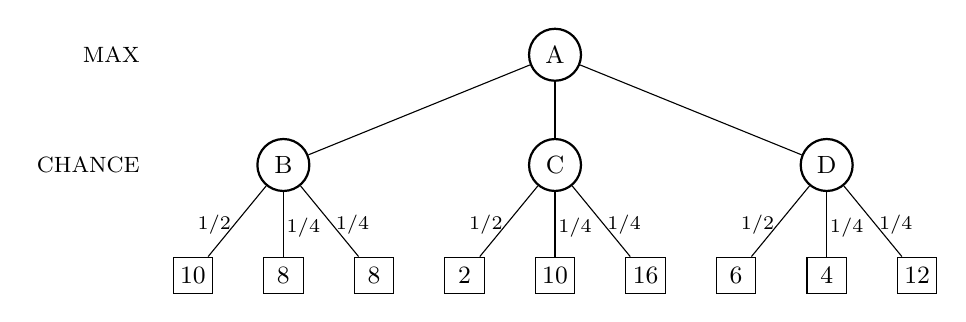
\begin{tikzpicture}[scale=1.0, every node/.style={transform shape}, gc/.style={draw, thick, circle, minimum size=6.6mm, inner sep=0pt, font=\small}, gl/.style={draw, rectangle, minimum width=5mm, minimum height=4.6mm, inner sep=1pt, font=\small}, gx/.style={draw=black!25, text=black!35}, val/.style={font=\footnotesize\bfseries, text=red!80!black, inner sep=1pt}]
\node[font=\footnotesize, anchor=east] at (-0.55,0.00) {MAX};
\node[font=\footnotesize, anchor=east] at (-0.55,-1.40) {CHANCE};
\node[gc] (n12) at (4.600,0.000) {A};
\node[gc] (n3) at (1.150,-1.400) {B};
\node[gl] (n0) at (0.000,-2.800) {10};
\node[gl] (n1) at (1.150,-2.800) {8};
\node[gl] (n2) at (2.300,-2.800) {8};
\node[gc] (n7) at (4.600,-1.400) {C};
\node[gl] (n4) at (3.450,-2.800) {2};
\node[gl] (n5) at (4.600,-2.800) {10};
\node[gl] (n6) at (5.750,-2.800) {16};
\node[gc] (n11) at (8.050,-1.400) {D};
\node[gl] (n8) at (6.900,-2.800) {6};
\node[gl] (n9) at (8.050,-2.800) {4};
\node[gl] (n10) at (9.200,-2.800) {12};
\draw (n12) -- (n3);
\draw (n12) -- (n7);
\draw (n12) -- (n11);
\draw (n3) -- (n0) node[pos=0.55, left, font=\scriptsize, inner sep=1pt]{$1/2$};
\draw (n3) -- (n1) node[pos=0.55, right, font=\scriptsize, inner sep=1pt]{$1/4$};
\draw (n3) -- (n2) node[pos=0.55, right, font=\scriptsize, inner sep=1pt]{$1/4$};
\draw (n7) -- (n4) node[pos=0.55, left, font=\scriptsize, inner sep=1pt]{$1/2$};
\draw (n7) -- (n5) node[pos=0.55, right, font=\scriptsize, inner sep=1pt]{$1/4$};
\draw (n7) -- (n6) node[pos=0.55, right, font=\scriptsize, inner sep=1pt]{$1/4$};
\draw (n11) -- (n8) node[pos=0.55, left, font=\scriptsize, inner sep=1pt]{$1/2$};
\draw (n11) -- (n9) node[pos=0.55, right, font=\scriptsize, inner sep=1pt]{$1/4$};
\draw (n11) -- (n10) node[pos=0.55, right, font=\scriptsize, inner sep=1pt]{$1/4$};
\end{tikzpicture}
\end{adjustbox}
\end{center}
\subq{(a)}Calculate the expectimax value of every node. Which move does MAX choose?
\begin{ansbox}[height=2.0cm]\end{ansbox}
\subq{(b)}Which move would MAX choose if the chance nodes were MIN nodes?
\begin{ansbox}[height=1.0cm]\end{ansbox}
\subq{(c)}Replace every leaf value $x$ by $x^2$ (order-preserving for these positive values). Does the expectimax decision change? What does this tell you about evaluation functions in stochastic games?
\begin{ansbox}[height=1.8cm]\end{ansbox}
\clearpage
\question{7}Consider the MCTS tree below; rollouts return 1 (win for the root player) or 0 (loss), $t$ is the total reward and $n$ the number of visits. Use $\mathrm{UCB1}=\bar V_i + C\sqrt{\ln N/n_i}$ with $C=\sqrt2$ (unvisited $=\infty$, ties to the left). A leaf never visited is rolled out directly; otherwise all its children are added and the rollout starts at the first. Expansions create: $A_1\to A_3,A_4$; $A_2\to A_5,A_6$; $B_1\to B_3,B_4$; $B_2\to B_5,B_6$; $C_1\to C_3,C_4$; $C_2\to C_5,C_6$.\begin{center}
\begin{adjustbox}{max width=\linewidth}
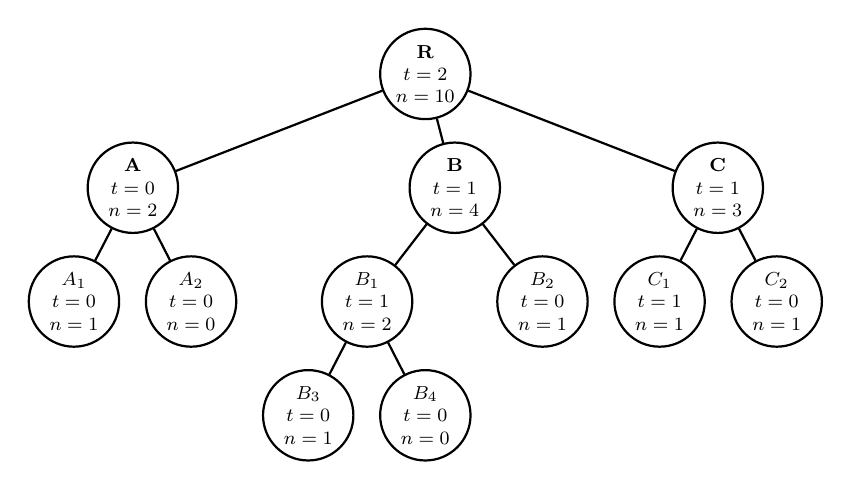
\begin{tikzpicture}[scale=0.85, every node/.style={transform shape}, mn/.style={draw, thick, circle, align=center, font=\footnotesize, inner sep=0.5pt, minimum size=13.5mm}]
\node[mn] (m1) at (5.25,0.00) {\textbf{R}\\ $t=2$\\ $n=10$};
\node[mn] (m2) at (0.88,-1.70) {\textbf{A}\\ $t=0$\\ $n=2$};
\node[mn] (m3) at (0.00,-3.40) {\textbf{$A_{1}$}\\ $t=0$\\ $n=1$};
\draw[thick] (m2) -- (m3);
\node[mn] (m4) at (1.75,-3.40) {\textbf{$A_{2}$}\\ $t=0$\\ $n=0$};
\draw[thick] (m2) -- (m4);
\draw[thick] (m1) -- (m2);
\node[mn] (m5) at (5.69,-1.70) {\textbf{B}\\ $t=1$\\ $n=4$};
\node[mn] (m6) at (4.38,-3.40) {\textbf{$B_{1}$}\\ $t=1$\\ $n=2$};
\node[mn] (m7) at (3.50,-5.10) {\textbf{$B_{3}$}\\ $t=0$\\ $n=1$};
\draw[thick] (m6) -- (m7);
\node[mn] (m8) at (5.25,-5.10) {\textbf{$B_{4}$}\\ $t=0$\\ $n=0$};
\draw[thick] (m6) -- (m8);
\draw[thick] (m5) -- (m6);
\node[mn] (m9) at (7.00,-3.40) {\textbf{$B_{2}$}\\ $t=0$\\ $n=1$};
\draw[thick] (m5) -- (m9);
\draw[thick] (m1) -- (m5);
\node[mn] (m10) at (9.62,-1.70) {\textbf{C}\\ $t=1$\\ $n=3$};
\node[mn] (m11) at (8.75,-3.40) {\textbf{$C_{1}$}\\ $t=1$\\ $n=1$};
\draw[thick] (m10) -- (m11);
\node[mn] (m12) at (10.50,-3.40) {\textbf{$C_{2}$}\\ $t=0$\\ $n=1$};
\draw[thick] (m10) -- (m12);
\draw[thick] (m1) -- (m10);
\end{tikzpicture}
\end{adjustbox}
\end{center}
\subq{(a)}Calculate UCB1 for $A$, $B$ and $C$. Which child is selected?
\begin{ansbox}[height=1.6cm]\end{ansbox}
\subq{(b)}Perform three iterations whose rollouts return $1,\ 0,\ 0$ (in order); update the statistics and draw the final tree.
\begin{ansbox}[height=8.0cm]\end{ansbox}
\subq{(c)}If the search stopped now, which move is played by the robust-child rule (the lecture's \texttt{best\_child})? Does the max-child rule agree?
\begin{ansbox}[height=1.2cm]\end{ansbox}
\clearpage
\question{8}This problem is about map colouring. Each region must be coloured Red (R), Green (G) or Blue (B), and neighbouring regions must have different colours. The constraint graph is shown below. The following questions are mutually independent.\begin{center}
\begin{adjustbox}{max width=\linewidth}
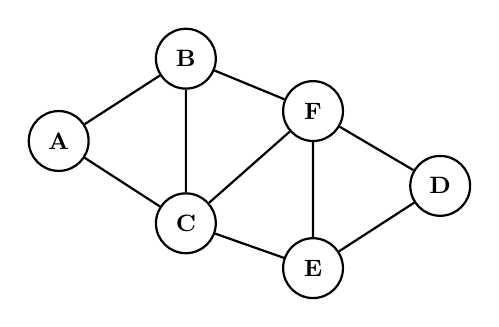
\begin{tikzpicture}[scale=0.95, every node/.style={transform shape}, cv/.style={draw, thick, circle, minimum size=8mm, inner sep=0pt, font=\small\bfseries}]
\node[cv] (A) at (0.00,1.00) {A};
\node[cv] (B) at (1.70,2.10) {B};
\node[cv] (C) at (1.70,-0.10) {C};
\node[cv] (F) at (3.40,1.40) {F};
\node[cv] (E) at (3.40,-0.70) {E};
\node[cv] (D) at (5.10,0.40) {D};
\draw[thick] (A) to[] (B);
\draw[thick] (A) to[] (C);
\draw[thick] (B) to[] (C);
\draw[thick] (B) to[] (F);
\draw[thick] (C) to[] (E);
\draw[thick] (C) to[] (F);
\draw[thick] (D) to[] (E);
\draw[thick] (D) to[] (F);
\draw[thick] (E) to[] (F);
\end{tikzpicture}
\end{adjustbox}
\end{center}
\subq{(a)}\textbf{Cross out} all values that would be eliminated by \emph{forward checking} after variable B has been assigned as shown.\begin{center}\small\begin{tabular}{|l|c|c|c|c|c|c|}\hline Variables & \textbf{A} & \textbf{B} & \textbf{C} & \textbf{D} & \textbf{E} & \textbf{F}\\ \hline Domains & R\ G\ B & \textbf{R} & R\ G\ B & R\ G\ B & R\ G\ B & R\ G\ B\\ \hline\end{tabular}\end{center}

\subq{(b)}A and B have been assigned as shown, but no constraint propagation has been done yet. \textbf{Cross out} all values that would be eliminated by \emph{arc consistency} (AC-3).\begin{center}\small\begin{tabular}{|l|c|c|c|c|c|c|}\hline Variables & \textbf{A} & \textbf{B} & \textbf{C} & \textbf{D} & \textbf{E} & \textbf{F}\\ \hline Domains & \textbf{R} & \textbf{G} & R\ G\ B & R\ G\ B & R\ G\ B & R\ G\ B\\ \hline\end{tabular}\end{center}

\subq{(c)}Variable A is already assigned and constraint propagation has been done. \textbf{Circle} all unassigned variables that might be selected by the \emph{Minimum-Remaining-Values} (MRV) heuristic.\begin{center}\small\begin{tabular}{|l|c|c|c|c|c|c|}\hline Variables & \textbf{A} & \textbf{B} & \textbf{C} & \textbf{D} & \textbf{E} & \textbf{F}\\ \hline Domains & \textbf{R} & G\ B & G\ B & R\ G\ B & R\ G\ B & R\ G\ B\\ \hline\end{tabular}\end{center}

\subq{(d)}Same situation. \textbf{Circle} all unassigned variables that might be selected by the \emph{Degree Heuristic}.\begin{center}\small\begin{tabular}{|l|c|c|c|c|c|c|}\hline Variables & \textbf{A} & \textbf{B} & \textbf{C} & \textbf{D} & \textbf{E} & \textbf{F}\\ \hline Domains & \textbf{R} & G\ B & G\ B & R\ G\ B & R\ G\ B & R\ G\ B\\ \hline\end{tabular}\end{center}

\subq{(e)}Assume no variable has been assigned yet. Solve the CSP using backtracking with \emph{forward checking}, choosing variables with MRV, then the degree heuristic (DH), and finally alphabetical order; try values in the order R, G, B. For every step give the MRV value of every region not yet coloured, and the DH values of the regions tied on the minimum MRV.
\par \underline{Step 1}\par\begin{center}\small \begin{tabular}{|l|c|c|c|c|c|c|}\hline Variables & \textbf{A} & \textbf{B} & \textbf{C} & \textbf{D} & \textbf{E} & \textbf{F}\\ \hline MRV & \phantom{0} & \phantom{0} & \phantom{0} & \phantom{0} & \phantom{0} & \phantom{0}\\[1mm]\hline DH & \phantom{0} & \phantom{0} & \phantom{0} & \phantom{0} & \phantom{0} & \phantom{0}\\[1mm]\hline\end{tabular}\end{center}Assign to the variable \rule{2.5cm}{0.3pt} with the value \rule{2.5cm}{0.3pt}\par
\underline{Step 2}\par\begin{center}\small \begin{tabular}{|l|c|c|c|c|c|c|}\hline Variables & \textbf{A} & \textbf{B} & \textbf{C} & \textbf{D} & \textbf{E} & \textbf{F}\\ \hline MRV & \phantom{0} & \phantom{0} & \phantom{0} & \phantom{0} & \phantom{0} & \phantom{0}\\[1mm]\hline DH & \phantom{0} & \phantom{0} & \phantom{0} & \phantom{0} & \phantom{0} & \phantom{0}\\[1mm]\hline\end{tabular}\end{center}Assign to the variable \rule{2.5cm}{0.3pt} with the value \rule{2.5cm}{0.3pt}\par
\underline{Step 3}\par\begin{center}\small \begin{tabular}{|l|c|c|c|c|c|c|}\hline Variables & \textbf{A} & \textbf{B} & \textbf{C} & \textbf{D} & \textbf{E} & \textbf{F}\\ \hline MRV & \phantom{0} & \phantom{0} & \phantom{0} & \phantom{0} & \phantom{0} & \phantom{0}\\[1mm]\hline DH & \phantom{0} & \phantom{0} & \phantom{0} & \phantom{0} & \phantom{0} & \phantom{0}\\[1mm]\hline\end{tabular}\end{center}Assign to the variable \rule{2.5cm}{0.3pt} with the value \rule{2.5cm}{0.3pt}\par
\underline{Step 4}\par\begin{center}\small \begin{tabular}{|l|c|c|c|c|c|c|}\hline Variables & \textbf{A} & \textbf{B} & \textbf{C} & \textbf{D} & \textbf{E} & \textbf{F}\\ \hline MRV & \phantom{0} & \phantom{0} & \phantom{0} & \phantom{0} & \phantom{0} & \phantom{0}\\[1mm]\hline DH & \phantom{0} & \phantom{0} & \phantom{0} & \phantom{0} & \phantom{0} & \phantom{0}\\[1mm]\hline\end{tabular}\end{center}Assign to the variable \rule{2.5cm}{0.3pt} with the value \rule{2.5cm}{0.3pt}\par
\underline{Step 5}\par\begin{center}\small \begin{tabular}{|l|c|c|c|c|c|c|}\hline Variables & \textbf{A} & \textbf{B} & \textbf{C} & \textbf{D} & \textbf{E} & \textbf{F}\\ \hline MRV & \phantom{0} & \phantom{0} & \phantom{0} & \phantom{0} & \phantom{0} & \phantom{0}\\[1mm]\hline DH & \phantom{0} & \phantom{0} & \phantom{0} & \phantom{0} & \phantom{0} & \phantom{0}\\[1mm]\hline\end{tabular}\end{center}Assign to the variable \rule{2.5cm}{0.3pt} with the value \rule{2.5cm}{0.3pt}\par
\underline{Step 6}\par Assign to the variable \rule{2.5cm}{0.3pt} with the value \rule{2.5cm}{0.3pt}\par
\subq{(f)}Now solve the CSP again with forward checking but \emph{without} MRV/DH: variables in the fixed order A, B, C, D, E, F and values in the order R, G, B. Draw the search tree and mark every node where forward checking empties a domain.
\begin{ansbox}[height=7.0cm]\end{ansbox}
\clearpage
\question{9}Variables $A,B,C\in\{1,\dots,6\}$ with the constraints $A=2B$, $B+C=7$ and $A<C$.
\subq{(a)}Run AC-3 starting from the queue $A\to B,\ B\to A,\ B\to C,\ C\to B,\ A\to C,\ C\to A$ (pop from the front; when $D_i$ shrinks, append every arc $X_k\to X_i$, $k\neq j$, not already queued). Show every revision.
\begin{ansbox}[height=5.0cm]\end{ansbox}
\subq{(b)}Cross out the eliminated values, and give all solutions.\begin{center}\small\begin{tabular}{|l|c|c|c|}\hline Variables & \textbf{A} & \textbf{B} & \textbf{C}\\ \hline Domains & 1\ 2\ 3\ 4\ 5\ 6 & 1\ 2\ 3\ 4\ 5\ 6 & 1\ 2\ 3\ 4\ 5\ 6\\ \hline\end{tabular}\end{center}
\begin{ansbox}[height=0.9cm]\end{ansbox}
\question{10}Answer the following questions briefly.
\subq{(a)}What is a rational agent? Using the lecture's examples (fingers on a hot stove; crossing at a crosswalk), distinguish a reflex action from an intelligent action. Can a reflex action be rational?
\begin{ansbox}[height=2.4cm]\end{ansbox}
\subq{(b)}What is abstraction in problem formulation? When is an abstraction valid and when is it useful? Illustrate with route finding in Romania.
\begin{ansbox}[height=2.4cm]\end{ansbox}
\subq{(c)}For 8-queens, compare the naive incremental formulation, the improved incremental formulation and the complete-state formulation used by hill climbing (size of the space / number of successors).
\begin{ansbox}[height=2.4cm]\end{ansbox}
\subq{(d)}List the four steps of an MCTS iteration and explain the difference between the tree policy and the default policy.
\begin{ansbox}[height=2.0cm]\end{ansbox}
\question{11}True or false?
For each statement, circle \textbf{T} or \textbf{F} and justify your answer in one or two sentences (an answer without a correct justification earns no credit).
\subq{1.}Tree-search DFS without any cycle checking is complete on every finite state space. \hfill \textbf{T \quad F}
\begin{ansbox}[height=1.5cm]\end{ansbox}
\subq{2.}Uniform-cost search is complete if every action cost is at least some $\epsilon>0$. \hfill \textbf{T \quad F}
\begin{ansbox}[height=1.5cm]\end{ansbox}
\subq{3.}Tree-search DFS needs only $O(bm)$ memory. \hfill \textbf{T \quad F}
\begin{ansbox}[height=1.5cm]\end{ansbox}
\subq{4.}Greedy best-first graph search is complete in finite state spaces. \hfill \textbf{T \quad F}
\begin{ansbox}[height=1.5cm]\end{ansbox}
\subq{5.}Weighted A* ($f=g+W\cdot h$, $W>1$) always returns an optimal path when $h$ is admissible. \hfill \textbf{T \quad F}
\begin{ansbox}[height=1.5cm]\end{ansbox}
\subq{6.}Minimax has time complexity $O(b^m)$ and space complexity $O(bm)$. \hfill \textbf{T \quad F}
\begin{ansbox}[height=1.5cm]\end{ansbox}
\subq{7.}An order-preserving transformation of the leaf values never changes the move chosen by expectimax. \hfill \textbf{T \quad F}
\begin{ansbox}[height=1.5cm]\end{ansbox}
\subq{8.}The robust child of the MCTS root is the child with the highest average reward. \hfill \textbf{T \quad F}
\begin{ansbox}[height=1.5cm]\end{ansbox}
\subq{9.}AC-3 runs in $O(cd^3)$ in the worst case. \hfill \textbf{T \quad F}
\begin{ansbox}[height=1.5cm]\end{ansbox}
\subq{10.}Forward checking makes the neighbours of the just-assigned variable consistent with it, but does not look further ahead. \hfill \textbf{T \quad F}
\begin{ansbox}[height=1.5cm]\end{ansbox}
\end{document}